\documentclass{article}
\usepackage{amssymb}
\usepackage{array}
\usepackage{amsmath}
\usepackage{subfigure}
\usepackage{tikz}
\usetikzlibrary{arrows,automata}
\newcounter{problem}
\newcounter{solution}
\newcounter{step}

\newcommand\Step{%
  \stepcounter{step}%
  \textbf{Step \thestep. }%
}

\newcommand\Problem{%
  \stepcounter{problem}%
  \textbf{\theproblem.}~%
  \setcounter{solution}{0}%
  \setcounter{step}{0}%
}

\newcommand\TheSolution{%
  \setcounter{step}{0}%
  \textbf{Solution \theproblem:}\\%
}

\newcommand\ASolution{%
  \setcounter{step}{0}%
  \stepcounter{solution}%
  \textbf{Solution \theproblem.\thesolution:}\\%
}
\parindent 0in
\parskip 1em
\begin{document}

\begin{center}
\fbox{\fbox{\parbox{4in}{\centering Assignment 4 by Lucas Karlsson}}}
\end{center}

\Problem Prove that $a^*(b+ab^*) = b + aa^*b^*.$

\TheSolution I read online about an algorithm to determine whether two RE are equal, one could construct 
NFA's from both and then using these convert them into DFA's using subset construction and then minimize 
these using a standard dfa minimization algorithm. And then compare these to see if they accpets the same 
language.

\Step Turning them into NFA's where \textbf{Q} = $a^*(b+ab^*)$ and \textbf{S} = $b+aa^*b^*$

\begin{center}
  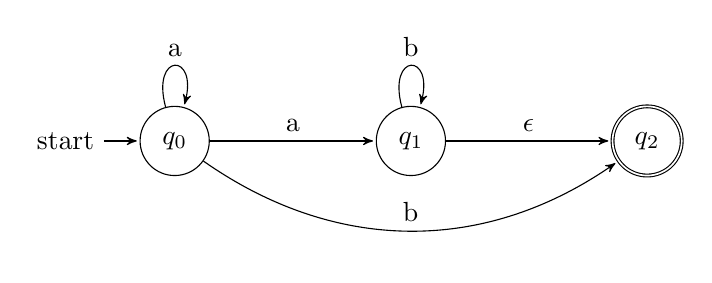
\begin{tikzpicture}[>=stealth',shorten >=1pt,auto,node distance=3cm]
    \node[initial,state]             (q0)                     {$q_0$};
    \node[state]           (q1) [right of=q0] {$q_1$};
    \node[accepting,state]                     (q2) [right of=q1] {$q_2$};

    \path[->] (q0) edge                node {a} (q1)
                   edge [loop above]   node {a} (q0)
                   edge [bend right=35] node {b} (q2)
              (q1) edge [loop above]   node {b} (q1)
                   edge                node {$\epsilon$} (q2);

  \end{tikzpicture}
\end{center}

\begin{center}
  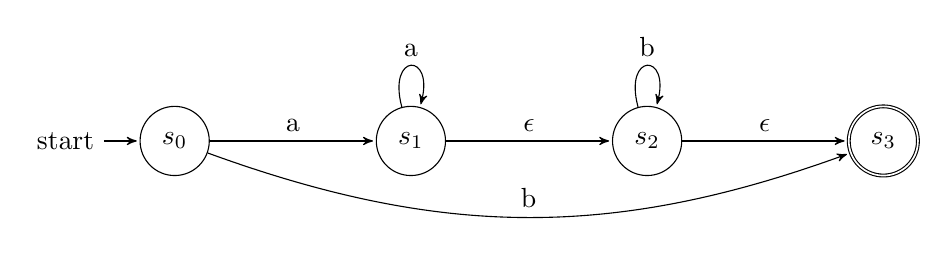
\begin{tikzpicture}[>=stealth',shorten >=1pt,auto,node distance=3cm]
    \node[initial,state]             (s0)               {$s_0$};
    \node[state]                     (s1) [right of=s0] {$s_1$};
    \node[state]                     (s2) [right of=s1] {$s_2$}; 
    \node[accepting,state]           (s3) [right of=s2] {$s_3$};

    \path[->] (s0) edge                 node {a} (s1)
                   edge [bend right=20] node {b} (s3)
              (s1) edge [loop above]    node {a} (s1)
                   edge                 node {$\epsilon$} (s2)
              (s2) edge                 node {$\epsilon$} (s3)
                   edge [loop above]    node {b} (s2);

  \end{tikzpicture}
\end{center}

\newpage
\Step Now we can turn these NFA's into DFA's by fist removing the epsilon transitions, this can be done
by everytime we have a state with a epsilon transition to another state, for every occurence of that first 
state we write both the first state and the state it had a epsilon transition to. I will keep on using
\textbf{Q} and \textbf{S} to represent my regular expression. Here are their tables first with epsilon 
transitions and then after I've removed them.

\begin{table}[h!]
  \centering
  \begin{tabular}{c c c c c}
         &&\textbf{$\epsilon$}&\textbf{a}&\textbf{b}\\ 
    $\to$    & $q_0$ & $\emptyset$ & $\{q_0, q_1\}$ & $q_2$\\
          & $q_1$ & $q_2$ & $\emptyset$ & $q_1$\\
\hfill *  & $q_2$ & $\emptyset$ & $\emptyset$ & $\emptyset$\\ [0.5ex]
\end{tabular} 
\begin{tabular}{|c c c c c}
            &&\textbf{$\epsilon$}&\textbf{a}&\textbf{b}\\ 
 $\to$       & $s_0$ & $\emptyset$ & $s_1$ & $s_3$\\
             & $s_1$ & $s_2$ & $s_1$ & $\emptyset$\\
             & $s_2$ & $s_3$ & $\emptyset$ & $s_2$\\
\hfill    *  & $s_3$ & $\emptyset$ & $\emptyset$ & $\emptyset$\\ [0.5ex]
\end{tabular}
\end{table}

\begin{table}[h!]
  \centering
  \begin{tabular}{c c c c}
         &&\textbf{a}&\textbf{b}\\ 
    $\to$    & $q_0$ & $\{q_0, q_1, q_2\}$ & $q_2$\\
             & $q_1$ & $\emptyset$ & $\{q_1,q_2\}$\\
\hfill *     & $q_2$ & $\emptyset$ & $\emptyset$\\ [0.5ex]
\end{tabular} 
\begin{tabular}{|c c c c}
            &&\textbf{a}&\textbf{b}\\ 
  $\to$       & $s_0$ & $\{s_1,s_2,s_3\}$ & $s_3$\\
             & $s_1$ & $\{s_1,s_2,s_3\}$ & $\emptyset$\\
             & $s_2$ & $\emptyset$ & $\{s_2,s_3\}$\\
\hfill    *  & $s_3$ & $\emptyset$ & $\emptyset$\\ [0.5ex]
\end{tabular}
\end{table}

\Step Now we can use the above table, the one without epsilon transitions to construct our DFA. The method
for this is quite simple but involves a lot of calculations. How this works is I'm going to start at 
\textbf{Q} and \textbf{S} initial state and from there expand by calculating $\delta (state, a or b) = 
\delta_n (state1, a or b) \cup \delta_n (state2, a or b) = \{states\}$ Where $\delta_n$ is the transition 
function for our NFA and $\delta$ is the transition function for our new DFA.

The calculations for our new \textbf{Q} DFA will be: \newline
$\delta(q_0,a) = \delta_n(q_0,a) = \{q_0,q_1,q_2\}$ \newline
$\delta(q_0,b) = \delta_n(q_0,b) = \{q_2\}$ \newline
$\delta(q_0q_1q_2, a) = \delta_n(q_0,a) \cup \delta_n(q_1,a) \cup \delta_n(q_2,a) = \{q_0,q_1,q_2\}$ \newline
$\delta(q_0q_1q_2, b) = \delta_n(q_0,b) \cup \delta_n(q_1,b) \cup \delta_n(q_2,b) = \{q_1,q_2\}$ \newline
$\delta(q_2,a) = \delta_n(q_2,a) = \{\emptyset\}$ \newline
$\delta(q_2,b) = \delta_n(q_2,b) = \{\emptyset\}$ \newline
$\delta(q_1q_2, a) = \delta_n(q_1,a) \cup \delta_n(q_2,a) = \{\emptyset\}$ \newline
$\delta(q_1q_2, b) = \delta_n(q_1,b) \cup \delta_n(q_2,b) = \{q_1,q_2\}$ \newline

The calculations for our new \textbf{S} DFA will be: \newline
$\delta(s_0, a) = \delta_n(s_0,a) = \{s_1,s_2,s_3\}$ \newline
$\delta(s_0, b) = \delta_n(s_0,b) = \{s_3\}$ \newline
$\delta(s_1s_2s_3, a) = \delta_n(s_1,a) \cup \delta_n(s_2,a) \cup \delta_n(s_3,a) = \{s_1,s_2,s_3\}$ \newline
$\delta(s_1s_2s_3, b) = \delta_n(s_1,b) \cup \delta_n(s_2,b) \cup \delta_n(s_3,b) = \{s_2,s_3\}$ \newline
$\delta(s_3, a) = \delta_n(s_3,a) = \{\emptyset\}$ \newline
$\delta(s_3, b) = \delta_n(s_3,b) = \{\emptyset\}$ \newline
$\delta(s_2s_3, a) = \delta_n(s_2,a) \cup \delta_n(s_3,a) = \{\emptyset\}$ \newline
$\delta(s_2s_3, b) = \delta_n(s_2,b) \cup \delta_n(s_3,b) = \{s_2,s_3\}$ \newline

This gives the new tables: 

\begin{table}[h!]
  \centering
\begin{tabular}{c c c c|}
       &&\textbf{a}&\textbf{b}\\ 
      \hfill $\to$ ($q_0$)  & $q_0$ & $q_0q_1q_2$ & $q_2$ \\ 
      \hfill *     ($q_1$)  & $q_0q_1q_2$ & $q_0q_1q_2$ & $q_1q_2$ \\ 
      \hfill *     ($q_2$)  & $q_2$ & $q_4$ & $q_4$ \\ 
      \hfill *     ($q_3$)  & $q_1q_2$ & $q_4$ & $q_1q_2$\\ 
      \hfill       ($q_4$)  & $q_4$ & $q_4$ & $q_4$ \\ [0.5ex]
    \end{tabular} 
\begin{tabular}{c c c c}
       &&\textbf{a}&\textbf{b}\\ 
      \hfill $\to$ ($s_0$)  & $s_0$ & $s_1s_2s_3$ & $s_3$ \\ 
      \hfill *     ($s_1$)  & $s_1s_2s_3$ & $s_1s_2s_3$ & $s_2s_3$ \\ 
      \hfill *     ($s_2$)  & $s_3$ & $s_4$ & $s_4$ \\ 
      \hfill *     ($s_3$)  & $s_2s_3$ & $s_4$ & $s_2s_3$\\ 
      \hfill       ($s_4$)  & $s_4$ & $s_4$ & $s_4$ \\ [0.5ex]
    \end{tabular} 
\
\end{table}

\Step we now have two identical tables that represent the same automaton and we have equality between 
\textbf{Q} and \textbf{S}. We can also see this automaton in the jflap file \textbf{ass4question1.jff}.

\newpage
\Problem Prove that every non regular language over an alphabet $\Sigma$ has an infinite
complement (with respect to $\Sigma^*$)

\TheSolution To start this off I will cite one of the regular languages closures that says "The complement of
a regular language is also regular" this implies that if we have the language $L$ which is regular, 
$\overline L$ which is the complement of $L$ will also by definition of the closure be regular. Another 
thing that is important that we also need to prove is that all finite languages are 
regular, this because regular languages are built recursively from our alphabet, this results in that every 
regular finite language can be represented by a automaton or a RE because the language will consist of a 
finite amount of string with a finite length. Clearly the finite language will always be regular. We can also
see this with a easy proof by contradiction:

If we assume the language $L$ is non-regular and defined as $L ={w_1,w_2,w_3,w_4...w_x}$ where $x \in 
\mathbb{N}$ we can contruct this language with the regular expression $w_1 + w_2 + w_3 + w_4 + .. + w_x$
and thus the language has to be regular, we have our contradiction.

Now we know that the non-regular language we are looking at will be infinite, now we need to prove that 
the complement to this language also will be infinite. This can be done by proving that the complement of
a non-regular language also will be non-regular. We can do this with the following calculation:

We assume that our language $L$ is non-regular, and that $\overline L$ is regular, that by the definition 
before would result in that $\overline {\overline L}$ would also be regular but $\overline {\overline L} = L$
and $L$ is non-regular. This translates into that if $L$ is non-regular then $\overline L$ is also non-
regular and every non-regular language is infinite with respect to $\Sigma^*$

\hfill
$\square$

\newpage
\Problem Show that the language $\{w \in \{0,1,2\}^* \mid \#_0(w) + \#_1(w) =  \#_2(w)\}$ over the 
alphabet $\{0,1,2\}$ is not regular by using the pumping lemma for regular languages. Here $\#_a(w)$ 
is the number of occurences of a in w.

\TheSolution 
We start by assuming that the language defined above, lets call it $L$, is regular. Then the pumping lemma
for regular languages will also apply for $L$.

\Step Let $n$ be the constant given by the pumping lemma 
and $w = 0^n1^n2^{2n}$, obviously $w \in L$ and $|w| \geqslant n$

\Step By the definition of the pumping lemma we know that $w = xyz$ with $|xy| \leqslant n$ and $y \neq 
\epsilon$

Because we chose $w$ the way we did we know that our $xy$ is located in the beginning of the word and 
that it is no longer than $n$, then $xy$ can only contain $0$'s. Because $y \neq \epsilon$ then $y$ should 
contain at least one $0$ and because $xy$ only contain $0$'s then $y$ will also contain only $0$'s.

\Step Let $x = 0^j$ for $j \geqslant 0$, $y = 0^i$ for $i \geqslant 1$ because $y \neq \epsilon$. and
$z = 0^{n-j-i}1^n2^{2n}$ our word will then be $w = 0^j0^i0^{n-i-j}1^n2^{2n}$ then for $k = 2$, the word
$xy^2z = xyyz = 0^j0^{2i}0^{n-j-i}1^n2^{2} = 0^{n+i}1^n2^{2n}$ will contain more $0$'s and $1$'s than $2's$ 
we can see that $n+i+n \geqslant 2n$ and then $xy^2z$ will not belong to $L$ which contradicts the pumping u
lemma therefore $L$ cannot be regular.

\newpage
\Problem Minimize the following DFA: (Do not just give the answer do a step by step)

\begin{table}[h!]
  \centering
  \begin{tabular}{c c c c}
    &&\textbf{0}&\textbf{1}\\ 
     \hfill $\to$ * & $s_0$ & $s_1$ & $s_3$\\
     \hfill         & $s_1$ & $s_4$ & $s_2$\\
     \hfill       * & $s_2$ & $s_1$ & $s_5$\\
     \hfill         & $s_3$ & $s_0$ & $s_4$\\
     \hfill         & $s_4$ & $s_4$ & $s_4$\\
     \hfill         & $s_5$ & $s_2$ & $s_4$\\[0.5ex]
  \end{tabular}
\end{table}

\TheSolution When minimizing a DFA you need to do two things, remove all states that cannot be reached. 
After that we partition the rest of the states so that every partition only contains states that are equal.
We can start by creating a automata from the given DFA, this because its easier to find equal states when 
we have visualized the transitions.

\begin{center}
  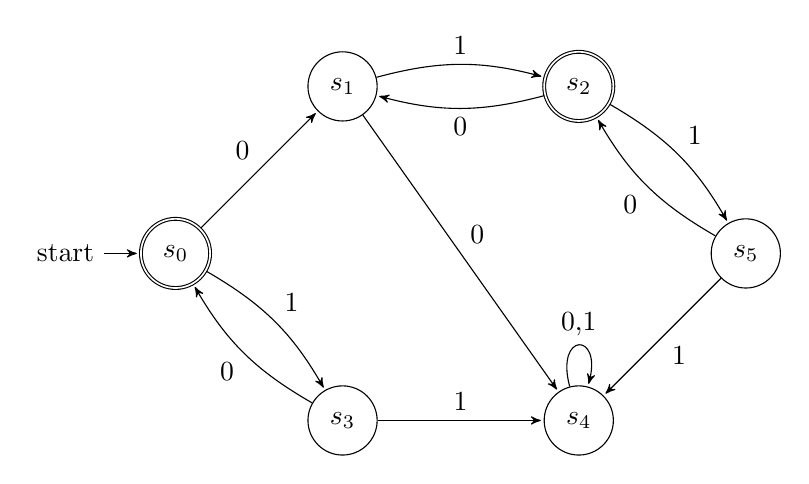
\begin{tikzpicture}[>=stealth',shorten >=1pt,auto,node distance=3cm]
    \node[accepting,initial,state] (s0)                     {$s_0$};
    \node[state]                   (s1) [above right of=s0] {$s_1$};
    \node[accepting,state]         (s2) [right of=s1]       {$s_2$};
    \node[state]                   (s3) [below right of=s0] {$s_3$};
    \node[state]                   (s4) [right of=s3]       {$s_4$};
    \node[state]                   (s5) [below right of=s2] {$s_5$};

    \path[->] (s0) edge                 node {0} (s1)
                   edge [bend left=15]  node {1} (s3)
              (s1) edge                 node {0} (s4)
                   edge [bend left=15]  node {1} (s2)
              (s2) edge [bend left=15]  node {0} (s1)
                   edge [bend left=15]  node {1} (s5)
              (s3) edge [bend left=15]  node {0} (s0)
                   edge                 node {1} (s4)
              (s4) edge [loop above]    node {0,1} (s4)
              (s5) edge [bend left=15]  node {0} (s2)
                   edge                 node {1} (s4);

  \end{tikzpicture}
\end{center}

\Step We create a table representing the DFA and the all the state tuples. The table will look like this:

\begin{center}
\begin{tabular}{l*{5}{|m{.2cm}}|}
	\cline{2-2}
	$s_1$&\\\cline{2-3}
	$s_2$&&\\\cline{2-4}
	$s_3$&&&\\\cline{2-5}
	$s_4$&&&&\\\cline{2-6}
	$s_5$&&&&&\\\cline{2-6}
 \multicolumn{1}{c}{}&
 \multicolumn{1}{c}{$s_0$}&
 \multicolumn{1}{c}{$s_1$}&
 \multicolumn{1}{c}{$s_2$}&
 \multicolumn{1}{c}{$s_3$}&
 \multicolumn{1}{c}{$s_4$}\\
\end{tabular}
\end{center}
\newpage
\Step Now we can start filling our table, firstly every pair where exactly one of the states is 
accepting. This because they cannot be equal.

\begin{center}
\begin{tabular}{l*{5}{|m{.2cm}}|}
	\cline{2-2}
	$s_1$&x\\\cline{2-3}
	$s_2$&&x\\\cline{2-4}
	$s_3$&x&&x\\\cline{2-5}
	$s_4$&x&&x&\\\cline{2-6}
	$s_5$&x&&x&&\\\cline{2-6}
 \multicolumn{1}{c}{}&
 \multicolumn{1}{c}{$s_0$}&
 \multicolumn{1}{c}{$s_1$}&
 \multicolumn{1}{c}{$s_2$}&
 \multicolumn{1}{c}{$s_3$}&
 \multicolumn{1}{c}{$s_4$}\\
\end{tabular}
\end{center}

\Step Now we have fewer states that we manually need to check. Lets start

$s_0,s_2$, $\delta (s_0, 0)$ and $\delta (s_2,0)$ both transition into the same state $s_1$
doing the other transition, $\delta (s_0,1)$ and $\delta (s_2,1)$ we see that they both go $(01)^*$
on $s_3$ and $s_5$ respectively and thus is equal again.

$s_1,s_3$ not equal because $\delta (s_1,0) = s_4$ and $\delta (s_3,0) = s_0$ and $s_4$ and $s_0$ is not
equal.

$s_1,s_4$ not equal because $\delta (s_1,1) = s_2$ and $\delta (s_4,1) = s_4$ and $s_2$ and $s_4$ is not
equal.

$s_1,s_5$ not equal because $\delta (s_1,1) = s_2$ and $\delta (s_5,1) = s_4$ and $s_2$ and $s_4$ is not
equal.

$s_3,s_4$ not equal because $\delta (s_3,0) = s_0$ and $\delta (s_4,0) = s_4$ and $s_0$ and $s_4$ is not
equal.

$s_3,s_5$ not equal because $\delta (s_3,0) = s_0$ and $\delta (s_5,0) = s_2$ and $s_0$ and $s_2$ is equal 
and $\delta (s_3,1) = s_4 = \delta (s_5,1)$ and these are also equal. $s_3, s_5$ is then equal!

$s_4,s_5$ not equal because $\delta (s_4,0) = s_4$ and $\delta (s_5,0) = s_2$ and $s_4$ and $s_2$ is not
equal.

Our table will then look like:

\begin{center}
\begin{tabular}{l*{5}{|m{.2cm}}|}
	\cline{2-2}
	$s_1$&x\\\cline{2-3}
	$s_2$&&x\\\cline{2-4}
	$s_3$&x&x&x\\\cline{2-5}
	$s_4$&x&x&x&x\\\cline{2-6}
	$s_5$&x&x&x&&x\\\cline{2-6}
 \multicolumn{1}{c}{}&
 \multicolumn{1}{c}{$s_0$}&
 \multicolumn{1}{c}{$s_1$}&
 \multicolumn{1}{c}{$s_2$}&
 \multicolumn{1}{c}{$s_3$}&
 \multicolumn{1}{c}{$s_4$}\\
\end{tabular}
\end{center}

\newpage
\Step We can now construct our minimized dfa, which can also be found in the jflap file 
\textbf{ass4question4.jff}

\begin{center}
  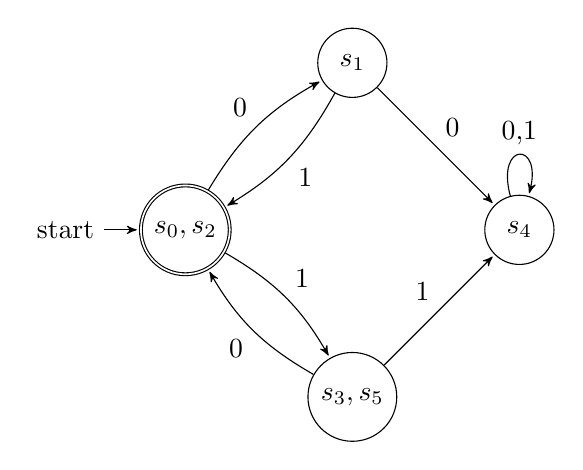
\begin{tikzpicture}[>=stealth',shorten >=1pt,auto,node distance=3cm]
    \node[accepting,initial,state] (s0)                     {$s_0,s_2$};
    \node[state]                   (s1) [above right of=s0] {$s_1$};
    \node[state]                   (s3) [below right of=s0] {$s_3,s_5$};
    \node[state]                   (s4) [below right of=s1]       {$s_4$};

    \path[->] (s0) edge [bend left=15]  node {0} (s1)
                   edge [bend left=15]  node {1} (s3)
              (s1) edge                 node {0} (s4)
                   edge [bend left=15]  node {1} (s0)
              (s3) edge [bend left=15]  node {0} (s0)
                   edge                 node {1} (s4)
              (s4) edge [loop above]    node {0,1} (s4);

  \end{tikzpicture}
\end{center}

\end{document}
